%% knit("diamond_neph_lfreq_model.Rnw")

\documentclass[12pt]{article}\usepackage[]{graphicx}\usepackage[]{color}
%% maxwidth is the original width if it is less than linewidth
%% otherwise use linewidth (to make sure the graphics do not exceed the margin)
\makeatletter
\def\maxwidth{ %
  \ifdim\Gin@nat@width>\linewidth
    \linewidth
  \else
    \Gin@nat@width
  \fi
}
\makeatother

\definecolor{fgcolor}{rgb}{0.345, 0.345, 0.345}
\newcommand{\hlnum}[1]{\textcolor[rgb]{0.686,0.059,0.569}{#1}}%
\newcommand{\hlstr}[1]{\textcolor[rgb]{0.192,0.494,0.8}{#1}}%
\newcommand{\hlcom}[1]{\textcolor[rgb]{0.678,0.584,0.686}{\textit{#1}}}%
\newcommand{\hlopt}[1]{\textcolor[rgb]{0,0,0}{#1}}%
\newcommand{\hlstd}[1]{\textcolor[rgb]{0.345,0.345,0.345}{#1}}%
\newcommand{\hlkwa}[1]{\textcolor[rgb]{0.161,0.373,0.58}{\textbf{#1}}}%
\newcommand{\hlkwb}[1]{\textcolor[rgb]{0.69,0.353,0.396}{#1}}%
\newcommand{\hlkwc}[1]{\textcolor[rgb]{0.333,0.667,0.333}{#1}}%
\newcommand{\hlkwd}[1]{\textcolor[rgb]{0.737,0.353,0.396}{\textbf{#1}}}%

\usepackage{framed}
\makeatletter
\newenvironment{kframe}{%
 \def\at@end@of@kframe{}%
 \ifinner\ifhmode%
  \def\at@end@of@kframe{\end{minipage}}%
  \begin{minipage}{\columnwidth}%
 \fi\fi%
 \def\FrameCommand##1{\hskip\@totalleftmargin \hskip-\fboxsep
 \colorbox{shadecolor}{##1}\hskip-\fboxsep
     % There is no \\@totalrightmargin, so:
     \hskip-\linewidth \hskip-\@totalleftmargin \hskip\columnwidth}%
 \MakeFramed {\advance\hsize-\width
   \@totalleftmargin\z@ \linewidth\hsize
   \@setminipage}}%
 {\par\unskip\endMakeFramed%
 \at@end@of@kframe}
\makeatother

\definecolor{shadecolor}{rgb}{.97, .97, .97}
\definecolor{messagecolor}{rgb}{0, 0, 0}
\definecolor{warningcolor}{rgb}{1, 0, 1}
\definecolor{errorcolor}{rgb}{1, 0, 0}
\newenvironment{knitrout}{}{} % an empty environment to be redefined in TeX

\usepackage{alltt}
\usepackage{times}
\usepackage{hyperref}
\usepackage{natbib}
\hypersetup{pdfpagemode=UseNone} % don't show bookmarks on initial view
\hypersetup{colorlinks, urlcolor={blue}}

% revise margins
\setlength{\headheight}{0.0in}
\setlength{\topmargin}{0.0in}
\setlength{\headsep}{0.0in}
\setlength{\textheight}{8.65in}
\setlength{\footskip}{0.35in}
\setlength{\oddsidemargin}{0.0in}
\setlength{\evensidemargin}{0.0in}
\setlength{\textwidth}{6.5in}

\setlength{\parskip}{6pt}
\setlength{\parindent}{0pt}

\title{A preliminary model for Quad-Rig catch comparison}
\author{For discussion only}
\date{}
\IfFileExists{upquote.sty}{\usepackage{upquote}}{}
\begin{document}



\maketitle
Methods for twin-rig catch comparison analysis are set out in \citet{Holst:Reville:2009}. Here, this model is preliminarily extended to greater than 2 cod-ends, in particular we focus on the quad-rig with 4 cod-ends. All treatment of the data is included as in a tutorial, which can be used as a basis for capacity building in the analysis of gear technology trials.

\section{Data}
The data used for this example come from the July 2014 diamond cod-end mesh size trials conducted by BIM aboard MFV Celtic Warrior II on the Smalls grounds. The data are read into R and processed as follows:

\begin{knitrout}\footnotesize
\definecolor{shadecolor}{rgb}{0.969, 0.969, 0.969}\color{fgcolor}\begin{kframe}
\begin{alltt}
\hlkwd{library}\hlstd{(gdata)}

\hlstd{neph.dat} \hlkwb{<-} \hlkwd{read.xls}\hlstd{(}\hlstr{"../data/Celtic Warrior Diamond mesh July 2014 Celtic Sea.xls"}\hlstd{,}
                     \hlkwc{sheet} \hlstd{=} \hlstr{"Nephrops Lengths"}\hlstd{,}
                     \hlkwc{stringsAsFactors} \hlstd{=} \hlnum{FALSE}\hlstd{)}

\hlcom{## remove Haul 22, as no recordings for 90mm }
\hlstd{neph.dat} \hlkwb{<-} \hlkwd{subset}\hlstd{(neph.dat, HAUL} \hlopt{!=} \hlnum{22}\hlstd{)}

\hlcom{## Show the first 2 rows}
\hlkwd{head}\hlstd{(neph.dat,} \hlnum{2}\hlstd{)}
\end{alltt}
\begin{verbatim}
##           Vessel       DATE HAUL COMPARTMENT Mesh.Size  SPECIES
## 1 Celtic Warrior 2014-07-19    1     Control      70mm Nephrops
## 2 Celtic Warrior 2014-07-19    1     Control      70mm Nephrops
##   Carapace.Length..mm.. COUNT SUBSRATIO
## 1                    16     1         1
## 2                    17    11         1
\end{verbatim}
\begin{alltt}
\hlcom{## Change the carapace length name}
\hlkwd{names}\hlstd{(neph.dat)[}\hlkwd{names}\hlstd{(neph.dat)} \hlopt{==} \hlstr{"Carapace.Length..mm.."}\hlstd{]} \hlkwb{<-} \hlstr{"Carapace.Length"}

\hlcom{## Make the "HAUL" variable character}
\hlstd{neph.dat}\hlopt{$}\hlstd{HAUL} \hlkwb{<-} \hlkwd{paste}\hlstd{(}\hlstr{"H"}\hlstd{, neph.dat}\hlopt{$}\hlstd{HAUL,} \hlkwc{sep} \hlstd{=}\hlstr{""}\hlstd{)}

\hlcom{## make some factor variables used in the analyses}
\hlstd{neph.dat}\hlopt{$}\hlstd{fHAUL} \hlkwb{<-} \hlkwd{factor}\hlstd{(neph.dat}\hlopt{$}\hlstd{HAUL,} \hlkwc{levels} \hlstd{=} \hlkwd{unique}\hlstd{(neph.dat}\hlopt{$}\hlstd{HAUL))}
\hlstd{neph.dat}\hlopt{$}\hlstd{fMesh.Size} \hlkwb{<-} \hlkwd{factor}\hlstd{(neph.dat}\hlopt{$}\hlstd{Mesh.Size,} \hlkwc{levels} \hlstd{=} \hlkwd{unique}\hlstd{(neph.dat}\hlopt{$}\hlstd{Mesh.Size))}

\hlcom{## remove observations above 99th and below 1th length percentile}
\hlcom{## these can be highly influential on the fits}
\hlstd{neph.dat} \hlkwb{<-} \hlkwd{subset}\hlstd{(neph.dat, Carapace.Length} \hlopt{<} \hlkwd{quantile}\hlstd{(Carapace.Length,} \hlnum{0.99}\hlstd{)} \hlopt{&}
                   \hlstd{Carapace.Length} \hlopt{>} \hlkwd{quantile}\hlstd{(Carapace.Length,} \hlnum{0.01}\hlstd{)}
                   \hlstd{)}
\end{alltt}
\end{kframe}
\end{knitrout}

Prepare the data for a multinomial fit.  

\begin{knitrout}\footnotesize
\definecolor{shadecolor}{rgb}{0.969, 0.969, 0.969}\color{fgcolor}\begin{kframe}
\begin{alltt}
\hlcom{## get count per length bin per haul by mesh size}
\hlcom{## using the reshape package (makes it easier to process data)}
\hlkwd{library}\hlstd{(reshape)}

\hlcom{## variables to keep }
\hlstd{vars2keep} \hlkwb{<-} \hlkwd{c}\hlstd{(}\hlstr{"fMesh.Size"}\hlstd{,} \hlstr{"Carapace.Length"}\hlstd{,} \hlstr{"fHAUL"}\hlstd{,} \hlstr{"COUNT"}\hlstd{)}

\hlcom{## melt the data frame}
\hlstd{neph.melt} \hlkwb{<-} \hlkwd{melt}\hlstd{(neph.dat[, vars2keep],}
                  \hlkwc{id} \hlstd{=} \hlkwd{c}\hlstd{(}\hlstr{"fMesh.Size"}\hlstd{,} \hlstr{"Carapace.Length"}\hlstd{,} \hlstr{"fHAUL"}\hlstd{))}

\hlcom{## re-form the dataframe in required format }
\hlstd{neph.cast} \hlkwb{<-} \hlkwd{cast}\hlstd{(neph.melt, Carapace.Length} \hlopt{+} \hlstd{fHAUL} \hlopt{~} \hlstd{fMesh.Size}  \hlopt{+} \hlstd{variable)}
\hlstd{neph.cast} \hlkwb{<-} \hlstd{neph.cast[}\hlkwd{order}\hlstd{(neph.cast}\hlopt{$}\hlstd{fHAUL, neph.cast}\hlopt{$}\hlstd{Carapace.Length), ]}
\hlstd{neph.cast[}\hlkwd{is.na}\hlstd{(neph.cast)]} \hlkwb{<-} \hlnum{0}

\hlcom{## show the first few rows}
\hlkwd{head}\hlstd{(neph.cast,} \hlnum{2}\hlstd{)}
\end{alltt}
\begin{verbatim}
##    Carapace.Length fHAUL 70mm_COUNT 80mm_COUNT 90mm_COUNT 100mm_COUNT
## 1               15    H1          0          2          1           0
## 24              16    H1          1          3          9           1
\end{verbatim}
\begin{alltt}
\hlcom{## format the subsampling ratio similarly}
\hlstd{vars2keep} \hlkwb{<-} \hlkwd{c}\hlstd{(}\hlstr{"fMesh.Size"}\hlstd{,} \hlstr{"fHAUL"}\hlstd{,} \hlstr{"SUBSRATIO"}\hlstd{)}

\hlstd{subs.melt} \hlkwb{<-} \hlkwd{melt}\hlstd{(}\hlkwd{unique}\hlstd{(neph.dat[, vars2keep]),} \hlkwc{id} \hlstd{=} \hlkwd{c}\hlstd{(}\hlstr{"fMesh.Size"}\hlstd{,} \hlstr{"fHAUL"}\hlstd{))}

\hlstd{subs.cast} \hlkwb{<-} \hlkwd{cast}\hlstd{(subs.melt, fHAUL}  \hlopt{~} \hlstd{fMesh.Size} \hlopt{+} \hlstd{variable)}

\hlcom{## merge counts and subsampling ratio back together }
\hlstd{neph.cast} \hlkwb{<-} \hlkwd{merge}\hlstd{(neph.cast, subs.cast,} \hlkwc{by} \hlstd{=} \hlstr{"fHAUL"}\hlstd{,} \hlkwc{all.x} \hlstd{=} \hlnum{TRUE}\hlstd{)}

\hlcom{## show first few lines}
\hlkwd{head}\hlstd{(neph.cast,} \hlnum{2}\hlstd{)}
\end{alltt}
\begin{verbatim}
##   fHAUL Carapace.Length 70mm_COUNT 80mm_COUNT 90mm_COUNT 100mm_COUNT
## 1    H1              15          0          2          1           0
## 2    H1              16          1          3          9           1
##   70mm_SUBSRATIO 80mm_SUBSRATIO 90mm_SUBSRATIO 100mm_SUBSRATIO
## 1              1              1              1               1
## 2              1              1              1               1
\end{verbatim}
\begin{alltt}
\hlcom{## Extract the matrix of counts}
\hlstd{count.vars} \hlkwb{<-} \hlkwd{c}\hlstd{(}\hlstr{"70mm_COUNT"}\hlstd{,} \hlstr{"80mm_COUNT"}\hlstd{,} \hlstr{"90mm_COUNT"}\hlstd{,} \hlstr{"100mm_COUNT"}\hlstd{)}

\hlstd{neph.count.mat} \hlkwb{<-} \hlkwd{as.matrix}\hlstd{(neph.cast[, count.vars])}

\hlkwd{colnames}\hlstd{(neph.count.mat)} \hlkwb{<-} \hlkwd{c}\hlstd{(}\hlstr{"70mm_COUNT"}\hlstd{,} \hlstr{"80mm_COUNT"}\hlstd{,} \hlstr{"90mm_COUNT"}\hlstd{,}
                              \hlstr{"100mm_COUNT"}\hlstd{)}

\hlcom{## Extract the matrix of subsampling ratios}
\hlstd{subsratio.vars} \hlkwb{<-} \hlkwd{c}\hlstd{(}\hlstr{"70mm_SUBSRATIO"}\hlstd{,} \hlstr{"80mm_SUBSRATIO"}\hlstd{,} \hlstr{"90mm_SUBSRATIO"}\hlstd{,}
                    \hlstr{"100mm_SUBSRATIO"}\hlstd{)}

\hlstd{subsratio.mat} \hlkwb{<-} \hlkwd{as.matrix}\hlstd{(neph.cast[, subsratio.vars])}

\hlcom{## Create the offset (NEED TO CHECK THIS)}
\hlstd{offset.mat} \hlkwb{<-} \hlkwd{log}\hlstd{(}\hlkwd{apply}\hlstd{(subsratio.mat,} \hlnum{2}\hlstd{,} \hlkwc{FUN} \hlstd{=}
                        \hlkwa{function}\hlstd{(}\hlkwc{zz}\hlstd{)\{zz}\hlopt{/}\hlstd{subsratio.mat[,}\hlnum{1}\hlstd{]\}))}
\end{alltt}
\end{kframe}
\end{knitrout}

Plot the data 
\begin{knitrout}\footnotesize
\definecolor{shadecolor}{rgb}{0.969, 0.969, 0.969}\color{fgcolor}\begin{kframe}
\begin{alltt}
\hlkwd{library}\hlstd{(ggplot2)}

\hlcom{## Get the proportions}
\hlstd{count.mesh} \hlkwb{<-} \hlkwd{as.matrix}\hlstd{(neph.cast[, count.vars])}

\hlstd{prop.mesh} \hlkwb{<-} \hlkwd{prop.table}\hlstd{(count.mesh,} \hlkwc{margin} \hlstd{=} \hlnum{1}\hlstd{)}

\hlstd{m} \hlkwb{<-} \hlkwd{dim}\hlstd{(prop.mesh)[}\hlnum{1}\hlstd{]}

\hlcom{## make a dataframe of the proportions for ggplot}
\hlstd{prop.mesh.df} \hlkwb{<-} \hlkwd{data.frame}\hlstd{(}
                  \hlkwc{Mesh.Size} \hlstd{=} \hlkwd{factor}\hlstd{(}\hlkwd{rep}\hlstd{(}\hlkwd{c}\hlstd{(}\hlstr{"70mm"}\hlstd{,} \hlstr{"80mm"}\hlstd{,} \hlstr{"90mm"}\hlstd{,} \hlstr{"100mm"}\hlstd{),}
                    \hlkwc{each} \hlstd{= m),} \hlkwc{levels} \hlstd{=} \hlkwd{c}\hlstd{(}\hlstr{"70mm"}\hlstd{,} \hlstr{"80mm"}\hlstd{,} \hlstr{"90mm"}\hlstd{,} \hlstr{"100mm"}\hlstd{)),}
                  \hlkwc{Carapace.Length} \hlstd{=} \hlkwd{rep}\hlstd{(neph.cast}\hlopt{$}\hlstd{Carapace.Length,} \hlkwc{times} \hlstd{=} \hlnum{4}\hlstd{),}
                  \hlkwc{proportion} \hlstd{=} \hlkwd{c}\hlstd{(prop.mesh),}
                  \hlkwc{count} \hlstd{=} \hlkwd{c}\hlstd{(count.mesh))}

\hlkwd{ggplot}\hlstd{(prop.mesh.df,} \hlkwd{aes}\hlstd{(}\hlkwc{x} \hlstd{= Carapace.Length,} \hlkwc{y} \hlstd{= proportion))} \hlopt{+}
  \hlkwd{geom_point}\hlstd{(}\hlkwc{colour} \hlstd{=} \hlstr{"#F8766D"}\hlstd{,} \hlkwc{alpha} \hlstd{=} \hlnum{0.2}\hlstd{,} \hlkwd{aes}\hlstd{(}\hlkwc{size} \hlstd{=} \hlkwd{log}\hlstd{(count)))} \hlopt{+}
  \hlkwd{facet_wrap}\hlstd{(}\hlopt{~} \hlstd{Mesh.Size)} \hlopt{+} \hlkwd{ylab}\hlstd{(}\hlstr{"Proportion of Nephrops per cod-end"}\hlstd{)}
\end{alltt}
\end{kframe}\begin{figure}
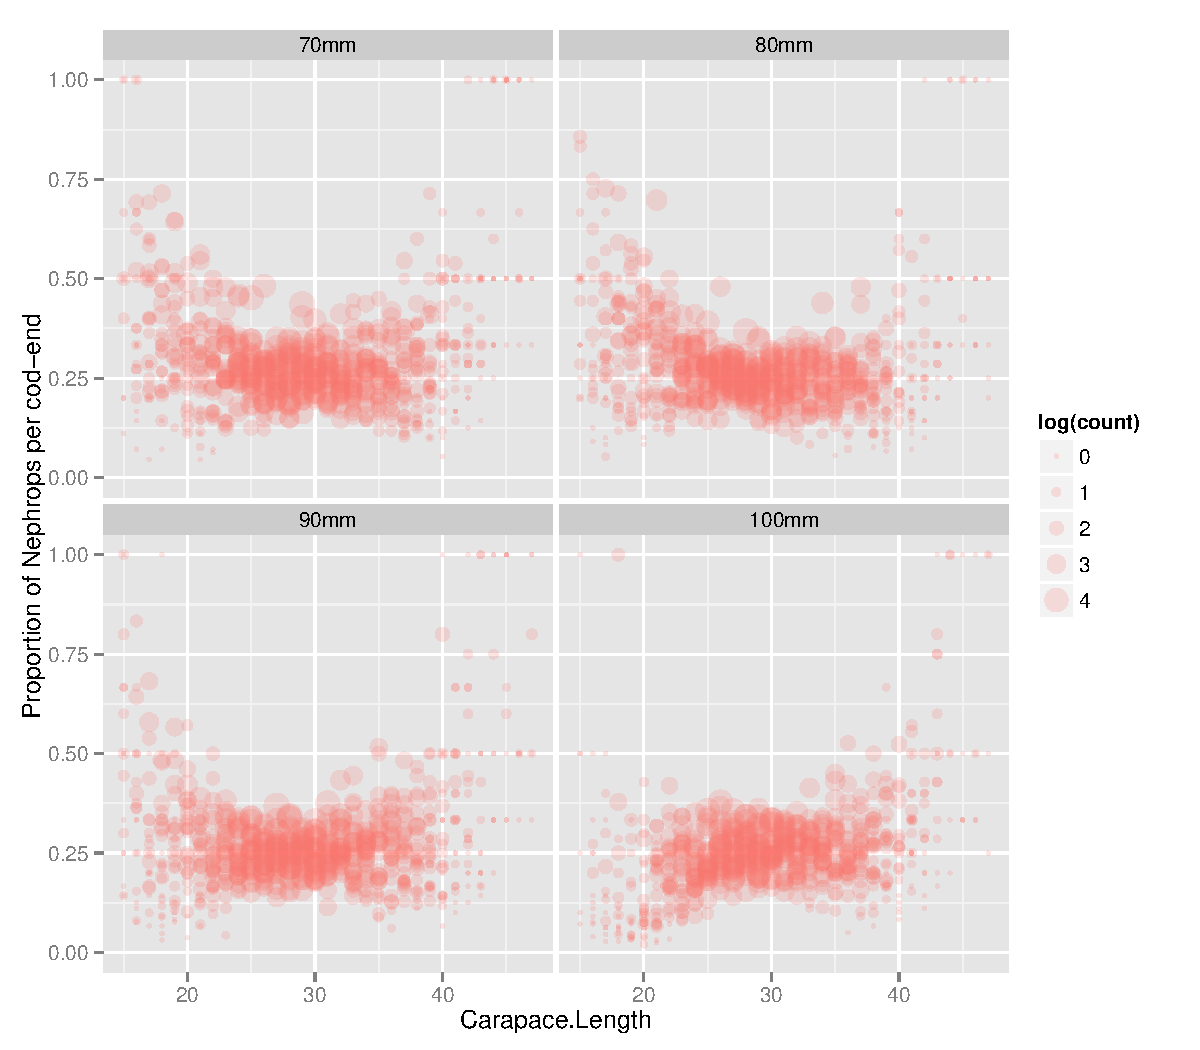
\includegraphics[width=\maxwidth]{figure/unnamed-chunk-4-1} \caption[Proportion of Nephrops catch retained per haul]{Proportion of Nephrops catch retained per haul. Each point represents the proportion of the Nephrops catch (in number) per haul and length class retained in a given cod-end (70mm, 80mm, 90mm, or 100mm). The size of the point is proportional to the log of the count.}\label{fig:unnamed-chunk-4}
\end{figure}


\end{knitrout}

\section{Model}
The model we focus on is the multinomial, which is a generalization of the binomial to cases with more than two categories (here 4 categories: 70mm, 80mm, 90mm, 100mm). Under the assumption that each net fishes the same, we would expect 25\% of the catch to be retained in each net. We can test that hypothesis.

\begin{knitrout}\footnotesize
\definecolor{shadecolor}{rgb}{0.969, 0.969, 0.969}\color{fgcolor}\begin{kframe}
\begin{alltt}
\hlkwd{library}\hlstd{(nnet)}

\hlcom{## First fit is constant proportions}
\hlcom{## not accounting for length}

\hlstd{mnom0} \hlkwb{<-} \hlkwd{multinom}\hlstd{(neph.count.mat} \hlopt{~} \hlnum{1} \hlopt{+} \hlkwd{offset}\hlstd{(offset.mat))}
\end{alltt}
\begin{verbatim}
## # weights:  24 (3 variable)
## initial  value 65833.303791 
## final  value 65796.538161 
## converged
\end{verbatim}
\begin{alltt}
\hlcom{## include carapace length }
\hlcom{## first scale it to range between zero and one}
\hlstd{max.length} \hlkwb{<-} \hlkwd{max}\hlstd{(neph.cast}\hlopt{$}\hlstd{Carapace.Length)}
\hlstd{neph.cast}\hlopt{$}\hlstd{Carapace.Length} \hlkwb{<-} \hlstd{neph.cast}\hlopt{$}\hlstd{Carapace.Length}\hlopt{/}\hlstd{max.length}

\hlcom{## Extend to third order polynomial (based on AIC and BIC)}
\hlstd{neph.cast}\hlopt{$}\hlstd{Carapace.Length2} \hlkwb{<-} \hlstd{neph.cast}\hlopt{$}\hlstd{Carapace.Length}\hlopt{^}\hlnum{2}
\hlstd{neph.cast}\hlopt{$}\hlstd{Carapace.Length3} \hlkwb{<-} \hlstd{neph.cast}\hlopt{$}\hlstd{Carapace.Length}\hlopt{^}\hlnum{3}

\hlcom{## }
\hlstd{mnom.length} \hlkwb{<-} \hlkwd{multinom}\hlstd{(neph.count.mat} \hlopt{~}
                        \hlstd{Carapace.Length} \hlopt{+} \hlstd{Carapace.Length2} \hlopt{+} \hlstd{Carapace.Length3} \hlopt{+}
                        \hlkwd{offset}\hlstd{(offset.mat),} \hlkwc{data} \hlstd{= neph.cast)}
\end{alltt}
\begin{verbatim}
## # weights:  36 (12 variable)
## initial  value 65833.303791 
## iter  10 value 65574.013563
## iter  20 value 65540.974075
## final  value 65538.628411 
## converged
\end{verbatim}
\begin{alltt}
\hlkwd{AIC}\hlstd{(mnom0, mnom.length)}
\end{alltt}
\begin{verbatim}
##             df      AIC
## mnom0        3 131599.1
## mnom.length 12 131101.3
\end{verbatim}
\end{kframe}
\end{knitrout}

Get predictions for the fitted model (note this is long-winded here but will be better coded for more than the preliminary example).

\begin{knitrout}\footnotesize
\definecolor{shadecolor}{rgb}{0.969, 0.969, 0.969}\color{fgcolor}\begin{kframe}
\begin{alltt}
\hlcom{## get predictions manually}
\hlcom{## CIs not defined in multinomial context but let's try}

\hlcom{## fit coefficients}
\hlstd{beta.mu} \hlkwb{<-} \hlkwd{c}\hlstd{(}\hlkwd{t}\hlstd{(}\hlkwd{coef}\hlstd{(mnom.length)))}

\hlcom{## fit coefficient variance covariance matrix}
\hlstd{Sigma} \hlkwb{<-} \hlkwd{vcov}\hlstd{(mnom.length)}

\hlcom{## number of lengths to predict for}
\hlstd{nlength} \hlkwb{<-} \hlnum{100}
\hlstd{pred.length} \hlkwb{<-} \hlkwd{seq}\hlstd{(}\hlkwd{min}\hlstd{(neph.cast}\hlopt{$}\hlstd{Carapace.Length),}
                   \hlkwd{max}\hlstd{(neph.cast}\hlopt{$}\hlstd{Carapace.Length),} \hlkwc{length} \hlstd{=} \hlnum{100}\hlstd{)}

\hlcom{## model matrix}
\hlstd{X} \hlkwb{<-} \hlkwd{cbind}\hlstd{(}\hlnum{1}\hlstd{, pred.length, pred.length}\hlopt{^}\hlnum{2}\hlstd{, pred.length}\hlopt{^}\hlnum{3}\hlstd{)}

\hlcom{## number of times to resample predictions to get CIs}
\hlstd{nresamp} \hlkwb{<-} \hlnum{100}
\hlstd{pred.array} \hlkwb{<-} \hlkwd{array}\hlstd{(}\hlnum{NA}\hlstd{,} \hlkwc{dim} \hlstd{=} \hlkwd{c}\hlstd{(nlength,} \hlnum{4}\hlstd{, nresamp))}

\hlcom{## package to draw from multivariate normal }
\hlkwd{library}\hlstd{(mvtnorm)}

\hlkwa{for}\hlstd{(i} \hlkwa{in} \hlnum{1}\hlopt{:}\hlstd{nresamp)\{}
  \hlcom{## print(i)}
  \hlstd{beta} \hlkwb{<-} \hlkwd{matrix}\hlstd{(}\hlkwd{rmvnorm}\hlstd{(}\hlnum{1}\hlstd{,} \hlkwc{mean} \hlstd{= beta.mu,} \hlkwc{sigma} \hlstd{= Sigma),}
                 \hlkwc{nrow} \hlstd{=} \hlnum{3}\hlstd{,} \hlkwc{byrow} \hlstd{=} \hlnum{TRUE}\hlstd{)}
  \hlstd{p80} \hlkwb{<-} \hlkwd{exp}\hlstd{(X} \hlopt \hlkwd{matrix}\hlstd{(beta[}\hlnum{1}\hlstd{,]))}\hlopt{/}\hlstd{(}\hlnum{1} \hlopt{+} \hlkwd{rowSums}\hlstd{(}\hlkwd{exp}\hlstd{(X} \hlopt \hlkwd{t}\hlstd{(beta))))}
  \hlstd{p90} \hlkwb{<-} \hlkwd{exp}\hlstd{(X} \hlopt \hlkwd{matrix}\hlstd{(beta[}\hlnum{2}\hlstd{,]))}\hlopt{/}\hlstd{(}\hlnum{1} \hlopt{+} \hlkwd{rowSums}\hlstd{(}\hlkwd{exp}\hlstd{(X} \hlopt \hlkwd{t}\hlstd{(beta))))}
  \hlstd{p100} \hlkwb{<-} \hlkwd{exp}\hlstd{(X} \hlopt \hlkwd{matrix}\hlstd{(beta[}\hlnum{3}\hlstd{,]))}\hlopt{/}\hlstd{(}\hlnum{1} \hlopt{+} \hlkwd{rowSums}\hlstd{(}\hlkwd{exp}\hlstd{(X} \hlopt \hlkwd{t}\hlstd{(beta))))}
  \hlstd{p70} \hlkwb{<-} \hlnum{1} \hlopt{-} \hlstd{p80} \hlopt{-} \hlstd{p90} \hlopt{-} \hlstd{p100}
  \hlstd{pred.p} \hlkwb{<-} \hlkwd{cbind}\hlstd{(p70, p80, p90, p100)}
  \hlstd{pred.array[ , , i]} \hlkwb{<-} \hlstd{pred.p}
  \hlkwd{rm}\hlstd{(pred.p)}
\hlstd{\}}

\hlcom{## mean across samples}
\hlstd{pred.mu} \hlkwb{<-} \hlkwd{apply}\hlstd{(pred.array,} \hlkwd{c}\hlstd{(}\hlnum{1}\hlstd{,} \hlnum{2}\hlstd{), mean)}

\hlcom{## upper across samples}
\hlstd{pred.upper} \hlkwb{<-} \hlkwd{apply}\hlstd{(pred.array,} \hlkwd{c}\hlstd{(}\hlnum{1}\hlstd{,} \hlnum{2}\hlstd{), quantile,} \hlkwc{p} \hlstd{=} \hlnum{0.975}\hlstd{)}

\hlcom{## lower across samples}
\hlstd{pred.lower} \hlkwb{<-} \hlkwd{apply}\hlstd{(pred.array,} \hlkwd{c}\hlstd{(}\hlnum{1}\hlstd{,} \hlnum{2}\hlstd{), quantile,} \hlkwc{p} \hlstd{=} \hlnum{0.025}\hlstd{)}

\hlcom{## bring all together in a data frame for ggplot}
\hlstd{m} \hlkwb{<-} \hlkwd{dim}\hlstd{(pred.mu)[}\hlnum{1}\hlstd{]}

\hlstd{pred.ci.df} \hlkwb{<-} \hlkwd{data.frame}\hlstd{(}
               \hlkwc{Mesh.Size} \hlstd{=} \hlkwd{factor}\hlstd{(}\hlkwd{rep}\hlstd{(}\hlkwd{c}\hlstd{(}\hlstr{"70mm"}\hlstd{,} \hlstr{"80mm"}\hlstd{,} \hlstr{"90mm"}\hlstd{,} \hlstr{"100mm"}\hlstd{),}
                 \hlkwc{each} \hlstd{= m),} \hlkwc{levels} \hlstd{=} \hlkwd{c}\hlstd{(}\hlstr{"70mm"}\hlstd{,} \hlstr{"80mm"}\hlstd{,} \hlstr{"90mm"}\hlstd{,} \hlstr{"100mm"}\hlstd{)),}
               \hlkwc{Carapace.Length} \hlstd{=} \hlkwd{rep}\hlstd{(pred.length} \hlopt{*} \hlstd{max.length,} \hlkwc{times} \hlstd{=} \hlnum{4}\hlstd{),}
               \hlkwc{proportion} \hlstd{=} \hlkwd{c}\hlstd{(pred.mu),}
               \hlkwc{lower} \hlstd{=} \hlkwd{c}\hlstd{(pred.lower),}
               \hlkwc{upper} \hlstd{=} \hlkwd{c}\hlstd{(pred.upper))}
\end{alltt}
\end{kframe}
\end{knitrout}

Finally overlay the fit on the sample proportions

\begin{knitrout}\footnotesize
\definecolor{shadecolor}{rgb}{0.969, 0.969, 0.969}\color{fgcolor}\begin{kframe}
\begin{alltt}
\hlstd{p} \hlkwb{<-} \hlkwd{ggplot}\hlstd{(prop.mesh.df,} \hlkwd{aes}\hlstd{(}\hlkwc{x} \hlstd{= Carapace.Length,} \hlkwc{y} \hlstd{= proportion))} \hlopt{+}
  \hlkwd{geom_point}\hlstd{(}\hlkwc{colour} \hlstd{=} \hlstr{"#F8766D"}\hlstd{,} \hlkwc{alpha} \hlstd{=} \hlnum{0.2}\hlstd{,} \hlkwd{aes}\hlstd{(}\hlkwc{size} \hlstd{=} \hlkwd{log}\hlstd{(count)))} \hlopt{+}
\hlkwd{facet_wrap}\hlstd{(}\hlopt{~} \hlstd{Mesh.Size)} \hlopt{+} \hlkwd{ylab}\hlstd{(}\hlstr{"Proportion of Nephrops per cod-end"}\hlstd{)}

\hlstd{p} \hlopt{+} \hlkwd{geom_ribbon}\hlstd{(}\hlkwc{data}\hlstd{=pred.ci.df,} \hlkwd{aes}\hlstd{(}\hlkwc{ymin} \hlstd{= lower,} \hlkwc{ymax} \hlstd{= upper),}
                \hlkwc{alpha}\hlstd{=}\hlnum{0.3}\hlstd{,} \hlkwc{fill} \hlstd{=} \hlstr{"blue"}\hlstd{)} \hlopt{+}
  \hlkwd{geom_line}\hlstd{(}\hlkwc{data} \hlstd{= pred.ci.df,} \hlkwd{aes}\hlstd{(}\hlkwc{x} \hlstd{= Carapace.Length,} \hlkwc{y} \hlstd{= proportion),}
            \hlkwc{col} \hlstd{=} \hlstr{"navy"}\hlstd{,} \hlkwc{size} \hlstd{=} \hlnum{0.5}\hlstd{)} \hlopt{+}
  \hlkwd{geom_hline}\hlstd{(}\hlkwd{aes}\hlstd{(}\hlkwc{yintercept} \hlstd{=} \hlnum{0.25}\hlstd{),} \hlkwc{linetype} \hlstd{=} \hlstr{"dashed"}\hlstd{)}
\end{alltt}
\end{kframe}\begin{figure}
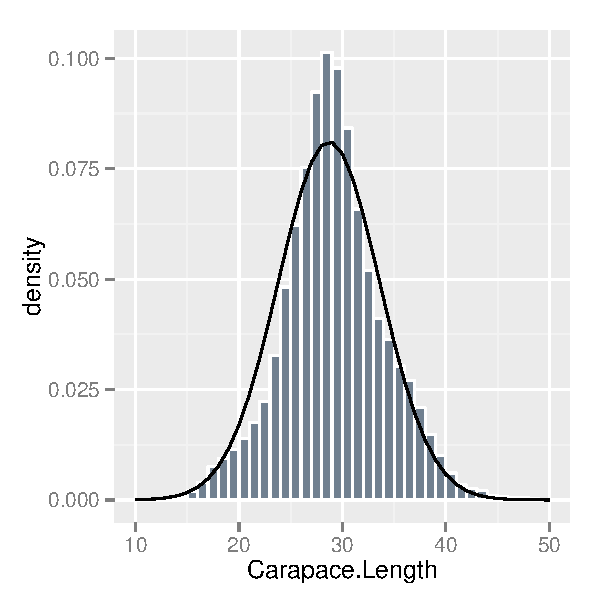
\includegraphics[width=\maxwidth]{figure/unnamed-chunk-7-1} \caption[Proportion of Nephrops catch retained per haul with fitted multinomial model and associated re-sampled intervals]{Proportion of Nephrops catch retained per haul with fitted multinomial model and associated re-sampled intervals. Null hypothesis of equal retention is displayed as the dashed line at 0.25.}\label{fig:unnamed-chunk-7}
\end{figure}


\end{knitrout}

\subsection{Including weight as a covariate}
Make a row per observation and merge with the weight data

\begin{knitrout}\footnotesize
\definecolor{shadecolor}{rgb}{0.969, 0.969, 0.969}\color{fgcolor}\begin{kframe}
\begin{alltt}
\hlcom{## get a row per length measurement (raise them also)}
\hlstd{n} \hlkwb{<-} \hlkwd{nrow}\hlstd{(neph.dat)}

\hlcom{##neph.dat2 <- neph.dat[rep(1:n, times = }
\hlcom{##                          round(neph.dat$COUNT/neph.dat$SUBSRATIO, 0)), ]}

\hlcom{## Note: no raising here}
\hlstd{neph.dat2} \hlkwb{<-} \hlstd{neph.dat[}\hlkwd{rep}\hlstd{(}\hlnum{1}\hlopt{:}\hlstd{n,} \hlkwc{times} \hlstd{= neph.dat}\hlopt{$}\hlstd{COUNT), ]}

\hlstd{weight.dat} \hlkwb{<-} \hlkwd{read.xls}\hlstd{(}\hlstr{"../data/Celtic Warrior Diamond mesh July 2014 Celtic Sea.xls"}\hlstd{,}
                       \hlkwc{sheet} \hlstd{=} \hlstr{"Weights"}\hlstd{,}
                       \hlkwc{stringsAsFactors} \hlstd{=} \hlnum{FALSE}\hlstd{)}

\hlcom{## Show the first 2 rows}
\hlkwd{head}\hlstd{(weight.dat,} \hlnum{2}\hlstd{)}
\end{alltt}
\begin{verbatim}
##         Date Haul.. Compartment Mesh.Size Species Total.weight..kg.
## 1 2014-07-19      1       TEST1      90mm    Bulk             26.28
## 2 2014-07-19      1       TEST1      90mm Haddock              0.38
##   Sbsample.weight..kg.
## 1                     
## 2
\end{verbatim}
\begin{alltt}
\hlcom{## create a new "HAUL" variable for the merge}
\hlstd{weight.dat}\hlopt{$}\hlstd{HAUL} \hlkwb{<-} \hlkwd{paste}\hlstd{(}\hlstr{"H"}\hlstd{, weight.dat}\hlopt{$}\hlstd{Haul..,} \hlkwc{sep} \hlstd{=}\hlstr{""}\hlstd{)}

\hlcom{## re-name total weight column}
\hlkwd{names}\hlstd{(weight.dat)[}\hlkwd{names}\hlstd{(weight.dat)} \hlopt{==} \hlstr{"Total.weight..kg."}\hlstd{]} \hlkwb{<-} \hlstr{"Total.Weight"}

\hlcom{## merge nephrops length and total bulk weight data}
\hlstd{neph.dat3} \hlkwb{<-} \hlkwd{merge}\hlstd{(neph.dat2,}
                   \hlkwd{subset}\hlstd{(weight.dat, Species} \hlopt{==} \hlstr{"Bulk"}\hlstd{)[,} \hlkwd{c}\hlstd{(}\hlstr{"Mesh.Size"}\hlstd{,} \hlstr{"HAUL"}\hlstd{,}
                                        \hlstr{"Total.Weight"}\hlstd{)],}
                   \hlkwc{by} \hlstd{=} \hlkwd{c}\hlstd{(}\hlstr{"Mesh.Size"}\hlstd{,} \hlstr{"HAUL"}\hlstd{))}

\hlstd{max.length} \hlkwb{<-} \hlkwd{max}\hlstd{(neph.dat3}\hlopt{$}\hlstd{Carapace.Length)}
\hlstd{neph.dat3}\hlopt{$}\hlstd{Carapace.Length} \hlkwb{<-} \hlstd{neph.dat3}\hlopt{$}\hlstd{Carapace.Length}\hlopt{/}\hlstd{max.length}
\hlstd{neph.dat3}\hlopt{$}\hlstd{Carapace.Length2} \hlkwb{<-} \hlstd{neph.dat3}\hlopt{$}\hlstd{Carapace.Length}\hlopt{^}\hlnum{2}
\hlstd{neph.dat3}\hlopt{$}\hlstd{Carapace.Length3} \hlkwb{<-} \hlstd{neph.dat3}\hlopt{$}\hlstd{Carapace.Length}\hlopt{^}\hlnum{3}
\end{alltt}
\end{kframe}
\end{knitrout}

Include weight in the fit

\begin{knitrout}\footnotesize
\definecolor{shadecolor}{rgb}{0.969, 0.969, 0.969}\color{fgcolor}\begin{kframe}
\begin{alltt}
\hlcom{## compare two ways of writing same model}
\hlcom{## in matrix format, as before except without offset for the moment}
\hlstd{mnom.length.matrix} \hlkwb{<-} \hlkwd{multinom}\hlstd{(neph.count.mat} \hlopt{~}
                               \hlstd{Carapace.Length} \hlopt{+}
                               \hlstd{Carapace.Length2} \hlopt{+}
                               \hlstd{Carapace.Length3,} \hlkwc{data} \hlstd{= neph.cast)}
\end{alltt}
\begin{verbatim}
## # weights:  20 (12 variable)
## initial  value 65846.209564 
## iter  10 value 65594.036234
## iter  20 value 65560.638668
## final  value 65558.314009 
## converged
\end{verbatim}
\begin{alltt}
\hlcom{## in long format (row per measurement)}
\hlstd{mnom.length.long} \hlkwb{<-} \hlkwd{multinom}\hlstd{(fMesh.Size} \hlopt{~}
                             \hlstd{Carapace.Length} \hlopt{+}
                             \hlstd{Carapace.Length2} \hlopt{+}
                             \hlstd{Carapace.Length3,} \hlkwc{data} \hlstd{= neph.dat3)}
\end{alltt}
\begin{verbatim}
## # weights:  20 (12 variable)
## initial  value 65846.209564 
## iter  10 value 65594.036234
## iter  20 value 65560.638668
## final  value 65558.314009 
## converged
\end{verbatim}
\begin{alltt}
\hlkwd{AIC}\hlstd{(mnom.length.matrix, mnom.length.long)}
\end{alltt}
\begin{verbatim}
##                    df      AIC
## mnom.length.matrix 12 131140.6
## mnom.length.long   12 131140.6
\end{verbatim}
\begin{alltt}
\hlcom{## Same model, now include bulk weight in long format model }
\hlcom{## in addition to carapace polynomials}

\hlstd{mnom.length.bulk} \hlkwb{<-} \hlkwd{multinom}\hlstd{(fMesh.Size} \hlopt{~}
                             \hlstd{Carapace.Length} \hlopt{+}
                             \hlstd{Carapace.Length2} \hlopt{+}
                             \hlstd{Carapace.Length3} \hlopt{+} \hlstd{Total.Weight,} \hlkwc{data} \hlstd{= neph.dat3)}
\end{alltt}
\begin{verbatim}
## # weights:  24 (15 variable)
## initial  value 65846.209564 
## iter  10 value 65467.670510
## iter  20 value 65392.143368
## iter  30 value 65389.022743
## iter  30 value 65389.022490
## iter  30 value 65389.022490
## final  value 65389.022490 
## converged
\end{verbatim}
\begin{alltt}
\hlkwd{AIC}\hlstd{(mnom.length.long, mnom.length.bulk)}
\end{alltt}
\begin{verbatim}
##                  df      AIC
## mnom.length.long 12 131140.6
## mnom.length.bulk 15 130808.0
\end{verbatim}
\begin{alltt}
\hlcom{## interaction between length and bulk}
\hlstd{mnom.length.bulk.inter} \hlkwb{<-} \hlkwd{multinom}\hlstd{(fMesh.Size} \hlopt{~}
                                   \hlstd{Carapace.Length} \hlopt{+}
                                   \hlstd{Carapace.Length2} \hlopt{+}
                                   \hlstd{Carapace.Length3} \hlopt{+}
                                   \hlstd{Total.Weight} \hlopt{+}
                                   \hlstd{Carapace.Length}\hlopt{:}\hlstd{Total.Weight} \hlopt{+}
                                   \hlstd{Carapace.Length2}\hlopt{:}\hlstd{Total.Weight} \hlopt{+}
                                   \hlstd{Carapace.Length3}\hlopt{:}\hlstd{Total.Weight}
                                   \hlstd{,} \hlkwc{data} \hlstd{= neph.dat3)}
\end{alltt}
\begin{verbatim}
## # weights:  36 (24 variable)
## initial  value 65846.209564 
## iter  10 value 65582.220539
## iter  20 value 65400.493488
## iter  30 value 65364.125707
## iter  40 value 65361.240613
## final  value 65361.182171 
## converged
\end{verbatim}
\begin{alltt}
\hlkwd{AIC}\hlstd{(mnom.length.bulk, mnom.length.bulk.inter)}
\end{alltt}
\begin{verbatim}
##                        df      AIC
## mnom.length.bulk       15 130808.0
## mnom.length.bulk.inter 24 130770.4
\end{verbatim}
\end{kframe}
\end{knitrout}

Get predictions for low, medium and high catch weights

\begin{knitrout}\footnotesize
\definecolor{shadecolor}{rgb}{0.969, 0.969, 0.969}\color{fgcolor}\begin{kframe}
\begin{alltt}
\hlstd{low.med.high.bulk} \hlkwb{<-} \hlkwd{quantile}\hlstd{(weight.dat[weight.dat}\hlopt{$}\hlstd{Species} \hlopt{==} \hlstr{"Bulk"}\hlstd{,]}\hlopt{$}\hlstd{Total.Weight,}
                              \hlkwc{p} \hlstd{=} \hlkwd{c}\hlstd{(}\hlnum{0.1}\hlstd{,} \hlnum{0.5}\hlstd{,} \hlnum{0.9}\hlstd{))}

\hlstd{pred.df} \hlkwb{<-} \hlkwd{expand.grid}\hlstd{(}\hlkwc{Carapace.Length} \hlstd{= pred.length,}
                       \hlkwc{Total.Weight} \hlstd{= low.med.high.bulk)}
\hlstd{pred.df}\hlopt{$}\hlstd{Carapace.Length2} \hlkwb{<-} \hlstd{pred.df}\hlopt{$}\hlstd{Carapace.Length}\hlopt{^}\hlnum{2}
\hlstd{pred.df}\hlopt{$}\hlstd{Carapace.Length3} \hlkwb{<-} \hlstd{pred.df}\hlopt{$}\hlstd{Carapace.Length}\hlopt{^}\hlnum{3}

\hlstd{mnom.pred} \hlkwb{<-} \hlkwd{predict}\hlstd{(mnom.length.bulk.inter,} \hlkwc{newdata} \hlstd{= pred.df,} \hlkwc{type} \hlstd{=} \hlstr{"prob"}\hlstd{)}

\hlstd{m} \hlkwb{<-} \hlkwd{dim}\hlstd{(mnom.pred)[}\hlnum{1}\hlstd{]}

\hlstd{mnom.pred.df} \hlkwb{<-} \hlkwd{data.frame}\hlstd{(}
                  \hlkwc{Mesh.Size} \hlstd{=} \hlkwd{factor}\hlstd{(}\hlkwd{rep}\hlstd{(}\hlkwd{c}\hlstd{(}\hlstr{"70mm"}\hlstd{,} \hlstr{"80mm"}\hlstd{,} \hlstr{"90mm"}\hlstd{,} \hlstr{"100mm"}\hlstd{),}
                    \hlkwc{each} \hlstd{= m),} \hlkwc{levels} \hlstd{=} \hlkwd{c}\hlstd{(}\hlstr{"70mm"}\hlstd{,} \hlstr{"80mm"}\hlstd{,} \hlstr{"90mm"}\hlstd{,} \hlstr{"100mm"}\hlstd{)),}
                  \hlkwc{Carapace.Length} \hlstd{=} \hlkwd{rep}\hlstd{(pred.df}\hlopt{$}\hlstd{Carapace.Length,} \hlkwc{times} \hlstd{=} \hlnum{4}\hlstd{),}
                  \hlkwc{Total.Weight} \hlstd{=} \hlkwd{rep}\hlstd{(pred.df}\hlopt{$}\hlstd{Total.Weight,} \hlkwc{times} \hlstd{=} \hlnum{4}\hlstd{),}
                  \hlkwc{proportion} \hlstd{=} \hlkwd{c}\hlstd{(mnom.pred))}

\hlstd{mnom.pred.df}\hlopt{$}\hlstd{Bulk.Weight} \hlkwb{<-}
  \hlkwd{ifelse}\hlstd{(mnom.pred.df}\hlopt{$}\hlstd{Total.Weight} \hlopt{==} \hlstd{low.med.high.bulk[}\hlnum{1}\hlstd{],} \hlstr{"Low"}\hlstd{,}
         \hlkwd{ifelse}\hlstd{(mnom.pred.df}\hlopt{$}\hlstd{Total.Weight} \hlopt{==} \hlstd{low.med.high.bulk[}\hlnum{2}\hlstd{],} \hlstr{"Medium"}\hlstd{,} \hlstr{"High"}\hlstd{)}
         \hlstd{)}


\hlstd{p} \hlopt{+} \hlkwd{geom_line}\hlstd{(}\hlkwc{data} \hlstd{= mnom.pred.df,}
              \hlkwd{aes}\hlstd{(}\hlkwc{x} \hlstd{= Carapace.Length}\hlopt{*}\hlstd{max.length,} \hlkwc{y} \hlstd{= proportion,}
                  \hlkwc{group} \hlstd{= Bulk.Weight,}
                  \hlkwc{colour} \hlstd{= Bulk.Weight))} \hlopt{+}
  \hlkwd{geom_hline}\hlstd{(}\hlkwd{aes}\hlstd{(}\hlkwc{yintercept} \hlstd{=} \hlnum{0.25}\hlstd{),} \hlkwc{linetype} \hlstd{=} \hlstr{"dashed"}\hlstd{)} \hlopt{+}
  \hlkwd{geom_vline}\hlstd{(}\hlkwd{aes}\hlstd{(}\hlkwc{xintercept} \hlstd{=} \hlnum{25}\hlstd{),} \hlkwc{linetype} \hlstd{=} \hlstr{"dashed"}\hlstd{)} \hlopt{+}
  \hlkwd{scale_colour_brewer}\hlstd{(}\hlkwc{palette}\hlstd{=}\hlstr{"Set1"}\hlstd{)}
\end{alltt}
\end{kframe}\begin{figure}
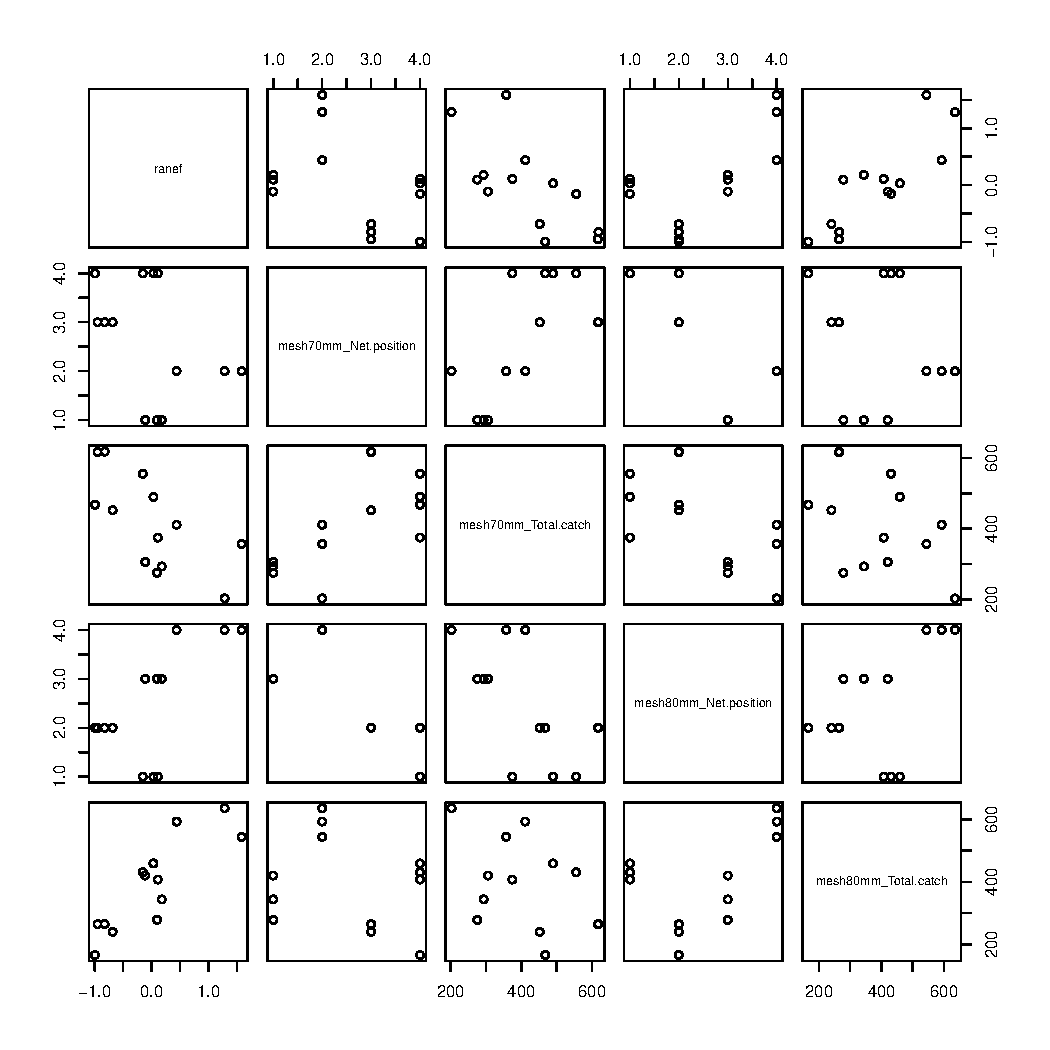
\includegraphics[width=\maxwidth]{figure/unnamed-chunk-10-1} \caption[Predicted influence of the bulk catch weight (low]{Predicted influence of the bulk catch weight (low: 26kg, medium: 61kg, high: 93kg) on the proportion of Nephrops catch retained per net. Null hypothesis of equal retention is displayed as the dashed line at 0.25. Minimum landing size of 25mm is shown as the vertical dashed line.}\label{fig:unnamed-chunk-10}
\end{figure}


\end{knitrout}

\bibliography{../../../../misc/epif_bibliography}
\bibliographystyle{../../../../misc/cjfas}
\end{document}

